\documentclass{standalone}
\usepackage{tikz-network}

\begin{document}
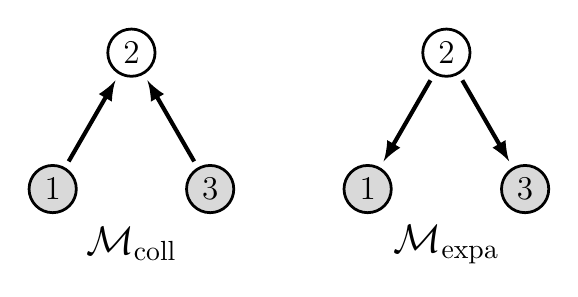
\begin{tikzpicture}

\SetVertexStyle[LineWidth=1, FillColor=black!15!white, LineColor=black, OuterSep=3, TextFont=\large]
\SetEdgeStyle[Color=black]
\SetTextStyle[TextFont=\Large]

\Vertex[x=4,label=1]{M1_1}
\Vertex[x=5,y=1.732,label=2,color=white]{M1_2}
\Vertex[x=6,label=3]{M1_3}
\Edge[Direct](M1_1)(M1_2)
\Edge[Direct](M1_3)(M1_2)
\Text[x=5,y=-0.7]{$\mathcal{M}_\mathrm{coll}$}

\Vertex[x=8,label=1]{M3_1}
\Vertex[x=9,y=1.732,label=2,color=white]{M3_2}
\Vertex[x=10,label=3]{M3_3}
\Edge[Direct](M3_2)(M3_1)
\Edge[Direct](M3_2)(M3_3)
\Text[x=9,y=-0.7]{$\mathcal{M}_\textrm{expa}$}

\end{tikzpicture}
\end{document}